\section*{NAIL062 V\&P Logika: 3. sada příkladů -- Algebra výroků, Problém SAT}
% po 3. přednášce

\subsection*{Cíle výuky:} Po absolvování cvičení student

    \begin{itemize}\setlength{\itemsep}{0pt}
        \item rozumí souvislosti výroků/teorií až na [$T$-]ekvivalenci a množin modelů (tzv. algebra výroků), umí aplikovat v konkrétních příkladech
        \item umí zakódovat daný problém jako instanci problému SAT
        \item získal praktickou zkušenost s použitím SAT solveru
        \item rozumí algoritmu pro řešení 2-SAT pomocí implikačního grafu (včetně nalezení všech modelů), umí aplikovat na příkladě
        \item rozumí algoritmu pro řešení Horn-SAT pomocí jednotkové propagace , umí aplikovat na příkladě
        \item rozumí algoritmu DPLL a umí jej aplikovat na příkladě
    \end{itemize}

\section*{Příklady na cvičení}


\begin{problem}

    Nechť $|\mathbb{P}|=n$ a mějme výrok $\varphi\in\mathrm{VF}_{\mathbb{P}}$ takový, že $|M(\varphi)|=k$. Určete počet až na ekvivalenci:
    \begin{enumerate}[(a)]
        \item výroků $\psi$ takových, že $\varphi \models \psi$ nebo $\psi \models \varphi$,
        \item teorií nad $\mathbb{P}$, ve kterých platí $\varphi$,
        \item kompletních teorií nad $\mathbb{P}$, ve kterých platí $\varphi$,
        \item teorií $T$ nad $\mathbb{P}$ takových, že $T \cup \{\varphi\}$ je bezesporná.
    \end{enumerate}
    Uvažme navíc spornou teorii $\{\varphi,\psi\}$ kde $|M(\psi)|=p$. Spočtěte až na ekvivalenci:
    \begin{enumerate}[(a)]\setcounter{enumi}{4}
        \item výroky $\chi$ takové, že $\varphi \vee \psi \models \chi$, 
        \item teorie, ve kterých platí $\varphi \vee \psi$.
    \end{enumerate}

    \begin{solution}
        \begin{enumerate}[(a)]
            \item Podmínku vyjádříme pomocí množin modelů: $\M(\varphi)\subseteq\M(\psi)$ nebo $\M(\psi)\subseteq\M(\varphi)$. Víme, že všech modelů je $2^n$, a $|\M(\varphi)|=k$. Chceme spočítat, kolik je možných množin $\M(\psi)$. Podmínku $\M(\varphi)\subseteq\M(\psi)$ splňuje $2^{2^n-k}$ množin (tj. tolik je nadmnožin dané $k$-prvkové množiny uvnitř $2^n$-prvkové množiny), podmínku $\M(\psi)\subseteq\M(\varphi)$ splňuje $2^k$ množin. Musíme ale být opatrní, abychom případ $\M(\psi)=\M(\varphi)$ nezapočítali dvakrát. Celkem máme $2^{2^n-k}+2^k-1$ možných množin modelů, tedy výroků $\psi$ až na ekvivalenci.
            \item $T\models\varphi$ právě když $\M(T)\subseteq\M(\varphi)$, takových množin $\M(T)$ je $2^k$
            \item Navíc máme podmínku $|\M(T)|=1$, 1-prvkových podmnožin $k$-prvkové množiny je $k$.
            \item Přeloženo do řeči modelů, podmínka říká, že $\M(T\cup\{\varphi\})\neq\emptyset$. Máme $\M(T\cup\{\varphi\})=\M(T,\varphi)=\M(T)\cap\M(\varphi)$ (jde o modely, ve kterých platí zároveň $T$ a $\varphi$). Počítáme tedy kolik možných množin $\M(T)$ má neprázdný průnik s $k$-prvkovou množinou $\M(\varphi)$. To lze vyjádřit např. jako $(2^k-1)\cdot(2^{2^n-k})$, kde $2^k-1$ je počet možných (neprázdných) ``průniků'' $\M(T)\cap\M(\varphi)$, a $2^{2^n-k}$ znamená, že pro modely, ve kterých neplatí $\varphi$, si můžeme libovolně zvolit, zda budou v naší množině.
            \item Protože $\{\varphi,\psi\}$ je sporná, víme, že $\emptyset=\M(\varphi,\psi)=\M(\varphi)\cap\M(\psi)$. Počítáme množiny $\M(\chi)$ takové, že $\M(\varphi\lor\psi)\subseteq\M(\chi)$. Díky Lindenbaum-Tarského algebře víme, že $\M(\varphi\lor\psi)=\M(\varphi)\cup\M(\psi)$. Z disjunktnosti máme $|\M(\varphi)\cup\M(\psi)|=k+p$, snadno spočítáme, že množných množin modelů $\M(\chi)$ je $2^{2^n-(k+p)}$.
            \item $\M(T)$ musí být podmnožinou $(k+p)$-prvkové $\M(\varphi\lor\psi)$, je jich tedy $2^{k+p}$.
        \end{enumerate}
                
    \end{solution}
    
\end{problem}


\begin{problem} \label{problem:2sat}
    
    Sestrojte implikační graf daného 2-CNF výroku. Je splnitelný? Pokud ano, najděte nějaké řešení: (a) výrok $\varphi$ níže, (b) $\varphi\land\neg p_1$, (c) $\varphi\land\neg p_1\land(p_1\lor p_2)$.
    $$
    \varphi=(p_1\vee \neg p_2)\wedge (p_2\vee p_3)\wedge (\neg p_3\vee \neg p_1)\wedge (\neg p_3\vee \neg p_4)\wedge (p_4\vee p_5)\wedge (\neg p_5\vee \neg p_1)
    $$

    \begin{solution}
        (a) Sestrojíme implikační graf. Zjistíme, že má dvě komponenty silné souvislosti: $C=\{p_1,p_2,\neg p_3,p_4,\neg p_5\}$ a $\overline{C}=\{\neg p_1,\neg p_2,p_3,\neg p_4,p_5\}$, nevede mezi nimi žádná hrana. Po kontrakci komponent tedy máme dvouvrcholový graf $\mathcal G^*$ bez hran, ten má dvě topologická uspořádání: $(C,\overline{C})$ a $(\overline{C},C)$, která odpovídají modelům $(0,0,1,0,1)$ a $(1,1,0,1,0)$.
        
        (b) Komponenty jsou stejné, ale do $\mathcal G^*$ přibude hrana $C\to\overline{C}$, tedy jediné topologické uspořádání je $(C,\overline{C})$, což odpovídá modelu $(0,0,1,0,1)$.

        (c) Implikační graf je nyní silně souvislý, tedy jeho jediná komponenta obsahuje (všechny) dvojice opačných literálů. To znamená, že výrok je nesplnitelný.
    \end{solution}

\end{problem}


\begin{problem}

    Pomocí jednotkové propagace zjistěte, zda je následující Hornův výrok splnitelný. Pokud ano, najděte nějaké splňující ohodnocení.
    \begin{align*}
        &(\neg p_1 \vee p_2 \vee \neg p_3)\wedge(\neg p_1 \vee p_2)\wedge p_1 \wedge (\neg p_1 \vee \neg p_2 \vee p_3)\wedge \\
        &(p_1\vee\neg p_2 \vee \neg p_4)\wedge(\neg p_2 \vee \neg p_3 \vee \neg p_4)\wedge(p_4\vee \neg p_5 \vee\neg p_6)
    \end{align*}

    \begin{solution}
        Provádíme postupně jednotkovou propagaci přes literály $p_1,p_2,p_3,\neg p_4$, zbývá výrok $\neg p_5\lor\neg p_6$. Ten stačí ohodnotit tak, aby alespoň jedna z výrokových proměnných $p_5,p_6$ byla ohodnocená nulou. Modely výroku jsou tedy: $\{(1,1,1,0,0,1),(1,1,1,0,1,0),(1,1,1,0,1,1)\}$                
    \end{solution}
    
\end{problem}


\begin{problem} \label{problem:dpll}

    Pomocí algoritmu DPLL rozhodněte, zda je následující CNF formule splnitelná:
    $$ 
    (\neg p_1 \lor \neg p_2)\land( \neg p_1 \lor p_2)\land( p_1 \lor \neg p_2)\land( p_2 \lor \neg p_3)\land( p_1 \lor p_3)
    $$

    \begin{solution}
        Výrok neobsahuje jednotkovou klauzuli ani literál s čistým výskytem, musíme tedy větvit, např. přes $p_1$:
        \begin{itemize}
            \item Z $\varphi\land p_1$ dostáváme po jednotkové propagaci
            $\neg p_2\land p_2\land( p_2 \lor \neg p_3)$, po jednotkové propagaci přes $\neg p_2$ dostáváme $\square\land\neg p_3$, což obsahuje prázdnou klauzuli $\square$, tedy je nesplnitelné.
            \item Z $\varphi\land \neg p_1$ dostáváme po jednotkové propagaci
            $\neg p_2\land( p_2 \lor \neg p_3)\land p_3$, po jednotkové propagaci přes $\neg p_2$ dostáváme $\neg p_3\land p_3$, po jednotkové propagaci přes $\neg p_3$ dostáváme prázdnou klauzuli $\square$, tedy opět je nesplnitelné.            
        \end{itemize}
        V obou (všech) větvích výpočtu jsme dokázali nesplnitelnost, výrok je tedy nesplnitelný.                        
    \end{solution}

\end{problem}


\begin{problem}

    Mějme daný orientovaný graf. Chceme zjistit, zda je acyklický, a pokud ano, nalézt nějaké jeho topologické uspořádání. Zakódujte tento problém do SAT.

    \begin{solution}
        Řešení jen naznačíme. Jako jazyk zvolme $\mathbb P=\{p_{uv}\mid u,v\in V\}$, kde $p_{uv}$ bude znamenat, že vrchol $u$ je v topologickém uspořádání (ostře) před $v$. To, že jde o ostré uspořádání, vyjádříme pomocí následujících axiomů:
        \begin{itemize}
            \item $\neg p_{vv}$ pro všechna $v\in V$
            \item $p_{uv}\limplies\neg p_{vu}$ pro všechna $u,v\in V$
            \item $p_{uv}\land p_{vw}\limplies p_{uw}$ pro všechna $u,v,w\in V$
        \end{itemize}
        Zbývá vyjádřit, že všechny grafové hrany vedou v topologickém uspořádání dopředu:
        \begin{itemize}
            \item $p_{uv}$ pro všechny hrany $(u,v)\in E$
        \end{itemize}
        Nakonec axiomy výše převedeme do CNF, v množinovém zápisu dostáváme:
        $$
        S=\{\{\neg p_{vv}\},\{\neg p_{uv},\neg p_{vu}\},\{\neg p_{uv},\neg p_{vw},\neg p_{uw}\} \mid u,v,w\in V\}\cup\{\{p_{uv}\}\mid(u,v)\in E\}
        $$
    \end{solution}

\end{problem}
    
    
\section*{Další příklady k procvičení}
    

\begin{problem}

    Uvažme následující výroky $\varphi$ a $\psi$ nad $\mathbb P=\{p, q, r, s\}$:
    \begin{align*}
        \varphi &= (\neg p \vee  q)\to(p\wedge r)\\
        \psi &= s\to q
    \end{align*}
    \begin{enumerate}[(a)]
        \item Určete počet (až na ekvivalenci) výroků $\chi$ nad $\mathbb P$ takových, že $\varphi\wedge\psi\models\chi$.
        \item Určete počet (až na ekvivalenci) úplných teorií $T$ nad $\mathbb P$ takových, že $T\models\varphi\wedge\psi$.
        \item Najděte nějakou axiomatizaci pro každou (až na ekvivalenci) kompletní teorii $T$ nad $\mathbb P$ takovou, že $T\models\varphi\wedge\psi$.
    \end{enumerate}

\end{problem}


\begin{problem} 
    
    Pomocí algoritmu jednotkové propagace najděte všechny modely:

    \begin{align*}
    &(\neg a \vee \neg b \vee c \vee \neg d)\wedge(\neg b \vee c)\wedge d \wedge (\neg a \vee \neg c \vee e)\wedge \\
    &(\neg c \vee \neg d)\wedge(\neg a \vee \neg d \vee \neg e)\wedge(a\vee \neg b \vee\neg e)
    \end{align*}

\end{problem}

    
\begin{problem} 
    
    Řešte pomocí implikačního grafu jako v Příkladu~\ref{problem:2sat}, a také pomocí algoritmu DPLL jako v Příkladu \ref{problem:dpll}:
    \begin{enumerate}[(a)]
        \item $(p_1\vee \neg p_2)\wedge (p_2\vee p_3)\wedge (\neg p_3\vee p_1)\wedge (\neg p_3\vee \neg p_4)\wedge (p_4\vee p_5)\wedge (\neg p_5\vee p_1)$
        \item $(p_0 \vee  p_2) \wedge  (p_0 \vee  \neg p_3) \wedge  (p_1 \vee  \neg p_3) 
        \wedge  (p_1 \vee  \neg p_4) \wedge  (p_2 \vee  \neg p_4) 
        \wedge  (p_0 \vee  \neg p_5)
        \wedge 
        (p_1 \vee  \neg p_5) \wedge  (p_2 \vee  \neg p_5) \wedge  (\neg p_1 \vee  \neg p_6) \wedge  (p_4 \vee  p_6) \wedge  (p_5 \vee  p_6) \wedge  p_1\wedge \neg p_7$
    \end{enumerate}

\end{problem}


\begin{problem}
    Lze obarvit čísla od 1 do $n$ dvěma barvami tak, že neexistuje monochromatické řešení rovnice
    $a+b=c$ pro žádná $1\leq a<b<c\leq n$? Sestrojte výrokovou formuli $\varphi_n$ v CNF která je splnitelná, právě když to lze. Zkuste nejprve $n=8$.
    
    Zkuste si doma: Napište skript generující $\varphi_n$ v DIMACS CNF formátu. Použijte SAT solver k nalezení nejmenšího $n$ pro které takové obarvení neexistuje (tj. každé 2-obarvení obsahuje monochromatickou trojici $a<b<c$ takovou, že $a+b=c$).
\end{problem}

    
\begin{problem}

    Věta o čtyřech barvách říká, že následující mapy lze obarvit 4 barvami tak, že žádné dva sousedící regiony nemají stejnou barvu. Najděte takové obarvení pomocí SAT solveru.
    \begin{multicols}{2}
    \begin{enumerate}[(a)]
        \item Mapa krajů Česka  
        
        \vfill 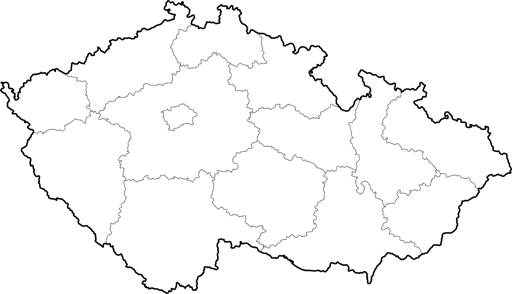
\includegraphics[width=0.5\textwidth]{files/map-coloring-czechia.png} \vfill
        
        \item Těžší instance  
        
        \vfill 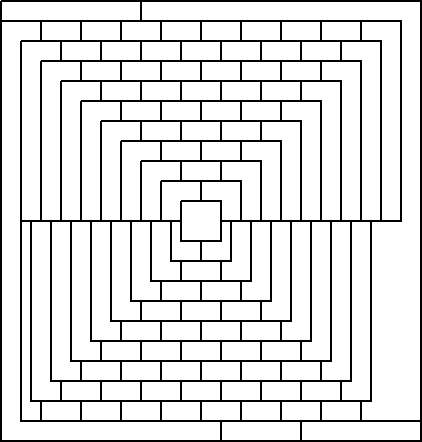
\includegraphics[width=0.33\textwidth]{files/map-coloring-hard.png} \vfill
    \end{enumerate}
    \end{multicols}

\end{problem}



\section*{K zamyšlení}
    
    
\begin{problem} 
    
    Pro danou formuli $\varphi$ v CNF najděte a 3-CNF formuli $\varphi'$ takovou, že $\varphi'$ je splnitelná, právě když $\varphi$ je splnitelná. Popište efektivní algoritmus konstrukce $\varphi'$ je-li dána $\varphi$ (tj. \emph{redukci} z problému SAT do problému 3-SAT).

\end{problem}


\begin{problem}
    Zakódujte problém setřídění dané $n$-tice celých čísel do SAT.
\end{problem}

\begin{problem}
    Zakódujte do SAT známou hádanku o farmáři, který potřebuje přepravit přes řeku vlka, kozu, a hlávku zelí.
\end{problem}
